\section{Descrizione proposta di stage}
\label{sez:descrizione-stage}

L'idea alla base dello stage è quella di riuscire ad automatizzare la creazione di un documento detto allegato tecnico; questo è un documento che contiene
tutte le informazioni tecniche riguardanti un progetto software, dalle tecnologie utilizzate alla struttura del progetto, passando per le scelte architetturali fino al piano di \textit{testing}.\\
L'azienda fino a questo momento ha sempre creato questo documento manualmente, ma con l'aumento dei progetti e delle risorse impiegate, la possibilità di usare un \textit{tool} che automatizzi questo processo,
almeno in parte, risulta molto interessante.\\

\noindent L'obiettivo dello stage è quindi quello di creare una piattaforma \textit{web} che permetta, tramite l'utilizzo di sistemi di \gls{ai-generativa}, di creare in modo automatico questo documento. \\
L'utente finale sarà un membro del \textit{team} di sviluppo od il \gls{project-manager}, che andrà a compilare dei \textit{Preset}, ovvero una lista di domande create \textit{ad-hoc} per raccogliere le informazioni necessarie per la creazione del documento,
ottimizzato in base al tipo di progetto che si vuole creare (una \textit{Web App}, una \textit {Mobile App,} ecc.).\\
Il sistema andrà quindi a creare il documento in automatico, tramite l'utilizzo di servizi di \gls{ai-generativa} forniti da AWS (AGGIUNGERE TERMINE GLOSSARIO). \\

\noindent L'utente potrà quindi andare a rigenerare il documento in parte o nella sua interezza, tramite l'inserimento di un \gls{prompt}.\\
Questo \gls{prompt} sarà una frase o un paragrafo che andrà a guidare il sistema nella creazione del documento, permettendo all'utente di specificare esattamente le migliorie che vuole vengano apportate al documento.\\
Tutte le versioni del documento verranno salvate e sarà possibile  visualizzare le differenze tra le varie versioni.\\
Quando l'utente sarà soddisfatto del documento creato, potrà scaricarlo in formato \textit{PDF}.\\
Nella {\hyperref[fig:project-schema]{Figura X}} è possibile vedere uno schema che rappresenta l'idea del progetto.\\

\begin{figure}[H]
    \label{fig:project-schema}
    \centering
    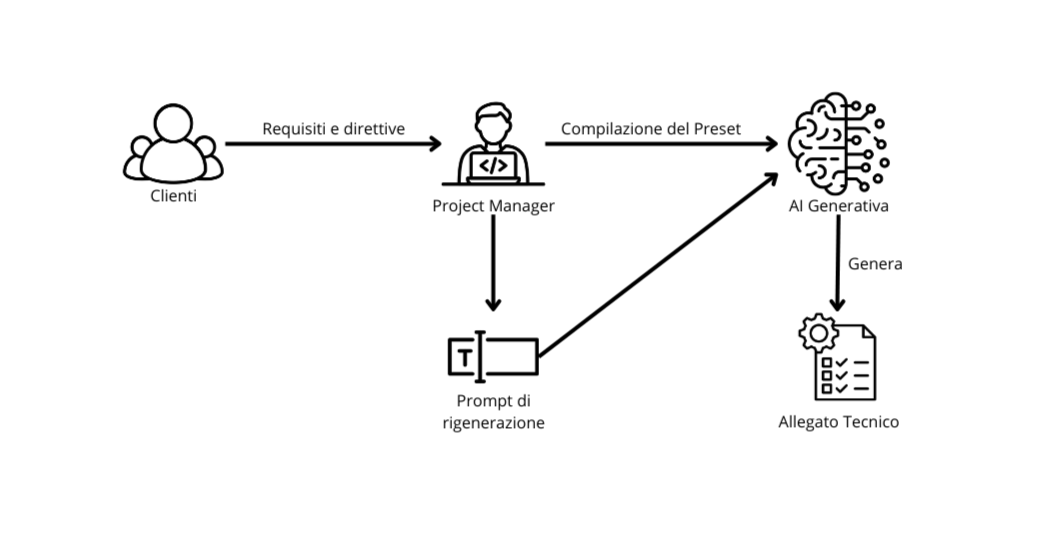
\includegraphics[scale=0.5]{gen-ai-documentation-schema.png}
    \caption{Schema del progetto}
\end{figure}